


% Header, overrides base

    % Make sure that the sphinx doc style knows who it inherits from.
    \def\sphinxdocclass{article}

    % Declare the document class
    \documentclass[letterpaper,10pt,english]{/usr/local/lib/python2.7/dist-packages/sphinx/texinputs/sphinxhowto}

    % Imports
    \usepackage[utf8]{inputenc}
    \DeclareUnicodeCharacter{00A0}{\\nobreakspace}
    \usepackage[T1]{fontenc}
    \usepackage{babel}
    \usepackage{times}
    \usepackage{import}
    \usepackage[Bjarne]{/usr/local/lib/python2.7/dist-packages/sphinx/texinputs/fncychap}
    \usepackage{longtable}
    \usepackage{/usr/local/lib/python2.7/dist-packages/sphinx/texinputs/sphinx}
    \usepackage{multirow}

    \usepackage{amsmath}
    \usepackage{amssymb}
    \usepackage{ucs}
    \usepackage{enumerate}

    % Used to make the Input/Output rules follow around the contents.
    \usepackage{needspace}

    % Pygments requirements
    \usepackage{fancyvrb}
    \usepackage{color}
    % ansi colors additions
    \definecolor{darkgreen}{rgb}{.12,.54,.11}
    \definecolor{lightgray}{gray}{.95}
    \definecolor{brown}{rgb}{0.54,0.27,0.07}
    \definecolor{purple}{rgb}{0.5,0.0,0.5}
    \definecolor{darkgray}{gray}{0.25}
    \definecolor{lightred}{rgb}{1.0,0.39,0.28}
    \definecolor{lightgreen}{rgb}{0.48,0.99,0.0}
    \definecolor{lightblue}{rgb}{0.53,0.81,0.92}
    \definecolor{lightpurple}{rgb}{0.87,0.63,0.87}
    \definecolor{lightcyan}{rgb}{0.5,1.0,0.83}

    % Needed to box output/input
    \usepackage{tikz}
        \usetikzlibrary{calc,arrows,shadows}
    \usepackage[framemethod=tikz]{mdframed}

    \usepackage{alltt}

    % Used to load and display graphics
    \usepackage{graphicx}
    \graphicspath{ {figs/} }
    \usepackage[Export]{adjustbox} % To resize

    % used so that images for notebooks which have spaces in the name can still be included
    \usepackage{grffile}


    % For formatting output while also word wrapping.
    \usepackage{listings}
    \lstset{breaklines=true}
    \lstset{basicstyle=\small\ttfamily}
    \def\smaller{\fontsize{9.5pt}{9.5pt}\selectfont}

    %Pygments definitions
    
\makeatletter
\def\PY@reset{\let\PY@it=\relax \let\PY@bf=\relax%
    \let\PY@ul=\relax \let\PY@tc=\relax%
    \let\PY@bc=\relax \let\PY@ff=\relax}
\def\PY@tok#1{\csname PY@tok@#1\endcsname}
\def\PY@toks#1+{\ifx\relax#1\empty\else%
    \PY@tok{#1}\expandafter\PY@toks\fi}
\def\PY@do#1{\PY@bc{\PY@tc{\PY@ul{%
    \PY@it{\PY@bf{\PY@ff{#1}}}}}}}
\def\PY#1#2{\PY@reset\PY@toks#1+\relax+\PY@do{#2}}

\expandafter\def\csname PY@tok@gd\endcsname{\def\PY@tc##1{\textcolor[rgb]{0.63,0.00,0.00}{##1}}}
\expandafter\def\csname PY@tok@gu\endcsname{\let\PY@bf=\textbf\def\PY@tc##1{\textcolor[rgb]{0.50,0.00,0.50}{##1}}}
\expandafter\def\csname PY@tok@gt\endcsname{\def\PY@tc##1{\textcolor[rgb]{0.00,0.27,0.87}{##1}}}
\expandafter\def\csname PY@tok@gs\endcsname{\let\PY@bf=\textbf}
\expandafter\def\csname PY@tok@gr\endcsname{\def\PY@tc##1{\textcolor[rgb]{1.00,0.00,0.00}{##1}}}
\expandafter\def\csname PY@tok@cm\endcsname{\let\PY@it=\textit\def\PY@tc##1{\textcolor[rgb]{0.25,0.50,0.50}{##1}}}
\expandafter\def\csname PY@tok@vg\endcsname{\def\PY@tc##1{\textcolor[rgb]{0.10,0.09,0.49}{##1}}}
\expandafter\def\csname PY@tok@m\endcsname{\def\PY@tc##1{\textcolor[rgb]{0.40,0.40,0.40}{##1}}}
\expandafter\def\csname PY@tok@mh\endcsname{\def\PY@tc##1{\textcolor[rgb]{0.40,0.40,0.40}{##1}}}
\expandafter\def\csname PY@tok@go\endcsname{\def\PY@tc##1{\textcolor[rgb]{0.53,0.53,0.53}{##1}}}
\expandafter\def\csname PY@tok@ge\endcsname{\let\PY@it=\textit}
\expandafter\def\csname PY@tok@vc\endcsname{\def\PY@tc##1{\textcolor[rgb]{0.10,0.09,0.49}{##1}}}
\expandafter\def\csname PY@tok@il\endcsname{\def\PY@tc##1{\textcolor[rgb]{0.40,0.40,0.40}{##1}}}
\expandafter\def\csname PY@tok@cs\endcsname{\let\PY@it=\textit\def\PY@tc##1{\textcolor[rgb]{0.25,0.50,0.50}{##1}}}
\expandafter\def\csname PY@tok@cp\endcsname{\def\PY@tc##1{\textcolor[rgb]{0.74,0.48,0.00}{##1}}}
\expandafter\def\csname PY@tok@gi\endcsname{\def\PY@tc##1{\textcolor[rgb]{0.00,0.63,0.00}{##1}}}
\expandafter\def\csname PY@tok@gh\endcsname{\let\PY@bf=\textbf\def\PY@tc##1{\textcolor[rgb]{0.00,0.00,0.50}{##1}}}
\expandafter\def\csname PY@tok@ni\endcsname{\let\PY@bf=\textbf\def\PY@tc##1{\textcolor[rgb]{0.60,0.60,0.60}{##1}}}
\expandafter\def\csname PY@tok@nl\endcsname{\def\PY@tc##1{\textcolor[rgb]{0.63,0.63,0.00}{##1}}}
\expandafter\def\csname PY@tok@nn\endcsname{\let\PY@bf=\textbf\def\PY@tc##1{\textcolor[rgb]{0.00,0.00,1.00}{##1}}}
\expandafter\def\csname PY@tok@no\endcsname{\def\PY@tc##1{\textcolor[rgb]{0.53,0.00,0.00}{##1}}}
\expandafter\def\csname PY@tok@na\endcsname{\def\PY@tc##1{\textcolor[rgb]{0.49,0.56,0.16}{##1}}}
\expandafter\def\csname PY@tok@nb\endcsname{\def\PY@tc##1{\textcolor[rgb]{0.00,0.50,0.00}{##1}}}
\expandafter\def\csname PY@tok@nc\endcsname{\let\PY@bf=\textbf\def\PY@tc##1{\textcolor[rgb]{0.00,0.00,1.00}{##1}}}
\expandafter\def\csname PY@tok@nd\endcsname{\def\PY@tc##1{\textcolor[rgb]{0.67,0.13,1.00}{##1}}}
\expandafter\def\csname PY@tok@ne\endcsname{\let\PY@bf=\textbf\def\PY@tc##1{\textcolor[rgb]{0.82,0.25,0.23}{##1}}}
\expandafter\def\csname PY@tok@nf\endcsname{\def\PY@tc##1{\textcolor[rgb]{0.00,0.00,1.00}{##1}}}
\expandafter\def\csname PY@tok@si\endcsname{\let\PY@bf=\textbf\def\PY@tc##1{\textcolor[rgb]{0.73,0.40,0.53}{##1}}}
\expandafter\def\csname PY@tok@s2\endcsname{\def\PY@tc##1{\textcolor[rgb]{0.73,0.13,0.13}{##1}}}
\expandafter\def\csname PY@tok@vi\endcsname{\def\PY@tc##1{\textcolor[rgb]{0.10,0.09,0.49}{##1}}}
\expandafter\def\csname PY@tok@nt\endcsname{\let\PY@bf=\textbf\def\PY@tc##1{\textcolor[rgb]{0.00,0.50,0.00}{##1}}}
\expandafter\def\csname PY@tok@nv\endcsname{\def\PY@tc##1{\textcolor[rgb]{0.10,0.09,0.49}{##1}}}
\expandafter\def\csname PY@tok@s1\endcsname{\def\PY@tc##1{\textcolor[rgb]{0.73,0.13,0.13}{##1}}}
\expandafter\def\csname PY@tok@sh\endcsname{\def\PY@tc##1{\textcolor[rgb]{0.73,0.13,0.13}{##1}}}
\expandafter\def\csname PY@tok@sc\endcsname{\def\PY@tc##1{\textcolor[rgb]{0.73,0.13,0.13}{##1}}}
\expandafter\def\csname PY@tok@sx\endcsname{\def\PY@tc##1{\textcolor[rgb]{0.00,0.50,0.00}{##1}}}
\expandafter\def\csname PY@tok@bp\endcsname{\def\PY@tc##1{\textcolor[rgb]{0.00,0.50,0.00}{##1}}}
\expandafter\def\csname PY@tok@c1\endcsname{\let\PY@it=\textit\def\PY@tc##1{\textcolor[rgb]{0.25,0.50,0.50}{##1}}}
\expandafter\def\csname PY@tok@kc\endcsname{\let\PY@bf=\textbf\def\PY@tc##1{\textcolor[rgb]{0.00,0.50,0.00}{##1}}}
\expandafter\def\csname PY@tok@c\endcsname{\let\PY@it=\textit\def\PY@tc##1{\textcolor[rgb]{0.25,0.50,0.50}{##1}}}
\expandafter\def\csname PY@tok@mf\endcsname{\def\PY@tc##1{\textcolor[rgb]{0.40,0.40,0.40}{##1}}}
\expandafter\def\csname PY@tok@err\endcsname{\def\PY@bc##1{\setlength{\fboxsep}{0pt}\fcolorbox[rgb]{1.00,0.00,0.00}{1,1,1}{\strut ##1}}}
\expandafter\def\csname PY@tok@kd\endcsname{\let\PY@bf=\textbf\def\PY@tc##1{\textcolor[rgb]{0.00,0.50,0.00}{##1}}}
\expandafter\def\csname PY@tok@ss\endcsname{\def\PY@tc##1{\textcolor[rgb]{0.10,0.09,0.49}{##1}}}
\expandafter\def\csname PY@tok@sr\endcsname{\def\PY@tc##1{\textcolor[rgb]{0.73,0.40,0.53}{##1}}}
\expandafter\def\csname PY@tok@mo\endcsname{\def\PY@tc##1{\textcolor[rgb]{0.40,0.40,0.40}{##1}}}
\expandafter\def\csname PY@tok@kn\endcsname{\let\PY@bf=\textbf\def\PY@tc##1{\textcolor[rgb]{0.00,0.50,0.00}{##1}}}
\expandafter\def\csname PY@tok@mi\endcsname{\def\PY@tc##1{\textcolor[rgb]{0.40,0.40,0.40}{##1}}}
\expandafter\def\csname PY@tok@gp\endcsname{\let\PY@bf=\textbf\def\PY@tc##1{\textcolor[rgb]{0.00,0.00,0.50}{##1}}}
\expandafter\def\csname PY@tok@o\endcsname{\def\PY@tc##1{\textcolor[rgb]{0.40,0.40,0.40}{##1}}}
\expandafter\def\csname PY@tok@kr\endcsname{\let\PY@bf=\textbf\def\PY@tc##1{\textcolor[rgb]{0.00,0.50,0.00}{##1}}}
\expandafter\def\csname PY@tok@s\endcsname{\def\PY@tc##1{\textcolor[rgb]{0.73,0.13,0.13}{##1}}}
\expandafter\def\csname PY@tok@kp\endcsname{\def\PY@tc##1{\textcolor[rgb]{0.00,0.50,0.00}{##1}}}
\expandafter\def\csname PY@tok@w\endcsname{\def\PY@tc##1{\textcolor[rgb]{0.73,0.73,0.73}{##1}}}
\expandafter\def\csname PY@tok@kt\endcsname{\def\PY@tc##1{\textcolor[rgb]{0.69,0.00,0.25}{##1}}}
\expandafter\def\csname PY@tok@ow\endcsname{\let\PY@bf=\textbf\def\PY@tc##1{\textcolor[rgb]{0.67,0.13,1.00}{##1}}}
\expandafter\def\csname PY@tok@sb\endcsname{\def\PY@tc##1{\textcolor[rgb]{0.73,0.13,0.13}{##1}}}
\expandafter\def\csname PY@tok@k\endcsname{\let\PY@bf=\textbf\def\PY@tc##1{\textcolor[rgb]{0.00,0.50,0.00}{##1}}}
\expandafter\def\csname PY@tok@se\endcsname{\let\PY@bf=\textbf\def\PY@tc##1{\textcolor[rgb]{0.73,0.40,0.13}{##1}}}
\expandafter\def\csname PY@tok@sd\endcsname{\let\PY@it=\textit\def\PY@tc##1{\textcolor[rgb]{0.73,0.13,0.13}{##1}}}

\def\PYZbs{\char`\\}
\def\PYZus{\char`\_}
\def\PYZob{\char`\{}
\def\PYZcb{\char`\}}
\def\PYZca{\char`\^}
\def\PYZam{\char`\&}
\def\PYZlt{\char`\<}
\def\PYZgt{\char`\>}
\def\PYZsh{\char`\#}
\def\PYZpc{\char`\%}
\def\PYZdl{\char`\$}
\def\PYZhy{\char`\-}
\def\PYZsq{\char`\'}
\def\PYZdq{\char`\"}
\def\PYZti{\char`\~}
% for compatibility with earlier versions
\def\PYZat{@}
\def\PYZlb{[}
\def\PYZrb{]}
\makeatother


    %Set pygments styles if needed...
    
        \definecolor{nbframe-border}{rgb}{0.867,0.867,0.867}
        \definecolor{nbframe-bg}{rgb}{0.969,0.969,0.969}
        \definecolor{nbframe-in-prompt}{rgb}{0.0,0.0,0.502}
        \definecolor{nbframe-out-prompt}{rgb}{0.545,0.0,0.0}

        \newenvironment{ColorVerbatim}
        {\begin{mdframed}[%
            roundcorner=1.0pt, %
            backgroundcolor=nbframe-bg, %
            userdefinedwidth=1\linewidth, %
            leftmargin=0.1\linewidth, %
            innerleftmargin=0pt, %
            innerrightmargin=0pt, %
            linecolor=nbframe-border, %
            linewidth=1pt, %
            usetwoside=false, %
            everyline=true, %
            innerlinewidth=3pt, %
            innerlinecolor=nbframe-bg, %
            middlelinewidth=1pt, %
            middlelinecolor=nbframe-bg, %
            outerlinewidth=0.5pt, %
            outerlinecolor=nbframe-border, %
            needspace=0pt
        ]}
        {\end{mdframed}}
        
        \newenvironment{InvisibleVerbatim}
        {\begin{mdframed}[leftmargin=0.1\linewidth,innerleftmargin=3pt,innerrightmargin=3pt, userdefinedwidth=1\linewidth, linewidth=0pt, linecolor=white, usetwoside=false]}
        {\end{mdframed}}

        \renewenvironment{Verbatim}[1][\unskip]
        {\begin{alltt}\smaller}
        {\end{alltt}}
    

    % Help prevent overflowing lines due to urls and other hard-to-break 
    % entities.  This doesn't catch everything...
    \sloppy

    % Document level variables
    \title{csv-parsing-plotting}
    \date{December 11, 2013}
    \release{}
    \author{Michele Pratusevich}
    \renewcommand{\releasename}{}

    % TODO: Add option for the user to specify a logo for his/her export.
    \newcommand{\sphinxlogo}{}

    % Make the index page of the document.
    \makeindex

    % Import sphinx document type specifics.
     


% Body

    % Start of the document
    \begin{document}

        
            \maketitle
        

        


        
        \section{Data analysis with Python}

What we want to do: draw an interesting conclusion from data. Go from
\href{http://www.amstat.org/publications/jse/datasets/30oysters.dat.txt}{table
of data} to a
\href{https://github.com/meet-projects/sample-YL1-individual-project/blob/master/oyster\_with\_titles.png}{picture
that tells us more}.

Steps:

\begin{enumerate}[1.]
\item
  Get data
\item
  Put data into Python
  \begin{enumerate}[1.]
  \item
    Use python \texttt{csv} package
  \item
    String parsing / formatting (turn into two lists of numbers)
  \end{enumerate}
\item
  Draw a plot / decide what plot to draw
  \begin{enumerate}[1.]
  \item
    matplotlib
  \end{enumerate}
\item
  Draw conclusions
\end{enumerate}
Big ideas: iteration, planning, big picture\paragraph{Definitions}

\begin{itemize}
\item
  \textbf{plot} - any picture that shows data in an interesting way
  (line graph, bar graph, histogram, etc.)
\item
  \textbf{graph} - same as a plot
\item
  \textbf{parsing} - getting useful information out of something. For
  example, getting the month out of the date string
\item
  \textbf{formatting} - turn something into a different way of
  representing (usually about strings). For example, turning dates from
  American format to European format
\end{itemize}\subsubsection{ipython notebook}

A \textbf{better} python shell. ``interactive python'' -- run one piece
of python at a time and see what happens. It's also in a web browser.

Run it from the folder in the terminal you want to save you work:

\begin{verbatim}
ipython notebook --pylab inline
\end{verbatim}
It will open Firefox and you'll edit python from there. (If you are
working on Windows, this is almost the same. Take a look at
\href{InstallipythonWindows.ipynb}{the Windows install instructions}
when you start the lab for more information.)\subsection{String parsing / formatting}

\textbf{Context}: computers can do some things better than humans. One
of these is change formats of strings. (e.g.~change date format from
American to European)

\textbf{Problem}: I run the American branch of the Red Cross. For every
patient that we treat I collect their birthday. I want to give this data
to my counterpart in France to compare the age demographic of our
patients. We have over 3 million records for the last year alone - I
need to change all the date formats before I send the data over.

2013-10-30 --\textgreater{} 2013-30-10

\begin{itemize}
\item
  By hand this is LONG AND TEDIOUS
\item
  By computer this is FAST AND EASY
\end{itemize}

    % Make sure that atleast 4 lines are below the HR
    \needspace{4\baselineskip}

    
        \vspace{6pt}
        \makebox[0.1\linewidth]{\smaller\hfill\tt\color{nbframe-in-prompt}In\hspace{4pt}{[}1{]}:\hspace{4pt}}\\*
        \vspace{-2.65\baselineskip}
        \begin{ColorVerbatim}
            \vspace{-0.7\baselineskip}
            \begin{Verbatim}[commandchars=\\\{\}]
\PY{c}{\PYZsh{} d is in form 2013\PYZhy{}10\PYZhy{}23 but we want}
\PY{c}{\PYZsh{} in form 2013\PYZhy{}23\PYZhy{}10}

\PY{n}{dates} \PY{o}{=} \PY{p}{[}\PY{l+s}{\PYZdq{}}\PY{l+s}{2013\PYZhy{}10\PYZhy{}30}\PY{l+s}{\PYZdq{}}\PY{p}{]}

\PY{k}{for} \PY{n}{d} \PY{o+ow}{in} \PY{n}{dates}\PY{p}{:}
	\PY{k}{print} \PY{l+s}{\PYZdq{}}\PY{l+s}{old = }\PY{l+s}{\PYZdq{}}\PY{p}{,} \PY{n}{d}
	\PY{n}{b} \PY{o}{=} \PY{n}{d}\PY{o}{.}\PY{n}{split}\PY{p}{(}\PY{l+s}{\PYZdq{}}\PY{l+s}{\PYZhy{}}\PY{l+s}{\PYZdq{}}\PY{p}{)}
	\PY{n}{new\PYZus{}date} \PY{o}{=} \PY{n}{b}\PY{p}{[}\PY{l+m+mi}{0}\PY{p}{]} \PY{o}{+} \PY{l+s}{\PYZdq{}}\PY{l+s}{\PYZhy{}}\PY{l+s}{\PYZdq{}} \PY{o}{+} \PY{n}{b}\PY{p}{[}\PY{l+m+mi}{2}\PY{p}{]} \PY{o}{+} \PY{l+s}{\PYZdq{}}\PY{l+s}{\PYZhy{}}\PY{l+s}{\PYZdq{}} \PY{o}{+} \PY{n}{b}\PY{p}{[}\PY{l+m+mi}{1}\PY{p}{]}
	\PY{k}{print} \PY{l+s}{\PYZdq{}}\PY{l+s}{new = }\PY{l+s}{\PYZdq{}}\PY{p}{,} \PY{n}{new\PYZus{}date}
\end{Verbatim}

            
                \vspace{-0.2\baselineskip}
            
        \end{ColorVerbatim}
    

    

        % If the first block is an image, minipage the image.  Else
        % request a certain amount of space for the input text.
        \needspace{4\baselineskip}
        
        

            % Add document contents.
            
                \begin{InvisibleVerbatim}
                \vspace{-0.5\baselineskip}
\begin{alltt}old =  2013-10-30
new =  2013-30-10
\end{alltt}

            \end{InvisibleVerbatim}
            
        
    
\subsection{When do you have these kinds of problems?}

\begin{itemize}
\item
  Modify LOTS of strings
\item
  Tables (of data) (like Excel sheets)
\item
  Move data from one storage to another (the example above)
\end{itemize}\subsection{How data is stored}

\begin{itemize}
\item
  csv = ``\textbf{C}omma-\textbf{S}eparated \textbf{V}alue''
\item
  store values in a text document, but special formatting for data (in a
  table)
\item
  sometimes the first row are ``headers'' (titles of columns)
\item
  a file format Python can understand
\item
  Example:
  \begin{itemize}
  \item
    \href{http://www.amstat.org/publications/jse/jse\_data\_archive.htm}{Data
    about oysters}
  \item
    \href{http://www.amstat.org/publications/jse/datasets/30oysters.dat.txt}{Save
    it as a csv}
  \end{itemize}
\end{itemize}\subsection{Getting data into Python}

Use the \textbf{csv} package. Here is a
\href{http://www.pythonforbeginners.com/systems-programming/using-the-csv-module-in-python/}{good
tutorial}. And here is a very simple
\href{https://github.com/meet-projects/sample-YL1-individual-project/blob/master/csv\_package\_demo.py}{example}.

    % Make sure that atleast 4 lines are below the HR
    \needspace{4\baselineskip}

    
        \vspace{6pt}
        \makebox[0.1\linewidth]{\smaller\hfill\tt\color{nbframe-in-prompt}In\hspace{4pt}{[}33{]}:\hspace{4pt}}\\*
        \vspace{-2.65\baselineskip}
        \begin{ColorVerbatim}
            \vspace{-0.7\baselineskip}
            \begin{Verbatim}[commandchars=\\\{\}]
\PY{k+kn}{import} \PY{n+nn}{csv}

\PY{c}{\PYZsh{} the name of the file}
\PY{c}{\PYZsh{} \PYZsq{}rb\PYZsq{} means \PYZdq{}for reading the file\PYZdq{}}
\PY{c}{\PYZsh{} (if you write \PYZsq{}wb\PYZsq{} that is }
\PY{c}{\PYZsh{} \PYZdq{}for writing the file\PYZdq{})}
\PY{n}{f} \PY{o}{=} \PY{n+nb}{open}\PY{p}{(}\PY{l+s}{\PYZsq{}}\PY{l+s}{30oysters.csv}\PY{l+s}{\PYZsq{}}\PY{p}{,} \PY{l+s}{\PYZsq{}}\PY{l+s}{rb}\PY{l+s}{\PYZsq{}}\PY{p}{)}

\PY{c}{\PYZsh{} the actual reader object that has the file}
\PY{n}{reader} \PY{o}{=} \PY{n}{csv}\PY{o}{.}\PY{n}{reader}\PY{p}{(}\PY{n}{f}\PY{p}{)}

\PY{c}{\PYZsh{}using this to count the row numbers}
\PY{n}{rownum} \PY{o}{=} \PY{l+m+mi}{0}

\PY{c}{\PYZsh{} the reader object is made of rows of data}
\PY{k}{for} \PY{n}{row} \PY{o+ow}{in} \PY{n}{reader}\PY{p}{:}
    
    \PY{c}{\PYZsh{} the header is the first row}
    \PY{k}{if} \PY{n}{rownum} \PY{o}{==} \PY{l+m+mi}{0}\PY{p}{:}
        \PY{n}{header} \PY{o}{=} \PY{n}{row}
    \PY{k}{else}\PY{p}{:}
        
        \PY{c}{\PYZsh{} for now just print the row}
        \PY{c}{\PYZsh{} later we will add more here}
        \PY{k}{print} \PY{n}{row}
    
    \PY{c}{\PYZsh{} count the row numbers}
    \PY{n}{rownum} \PY{o}{+}\PY{o}{=} \PY{l+m+mi}{1}

\PY{c}{\PYZsh{} you always must close your file,}
\PY{c}{\PYZsh{} or you will use too much memory}
\PY{n}{f}\PY{o}{.}\PY{n}{close}\PY{p}{(}\PY{p}{)}
\end{Verbatim}

            
                \vspace{-0.2\baselineskip}
            
        \end{ColorVerbatim}
    

    

        % If the first block is an image, minipage the image.  Else
        % request a certain amount of space for the input text.
        \needspace{4\baselineskip}
        
        

            % Add document contents.
            
                \begin{InvisibleVerbatim}
                \vspace{-0.5\baselineskip}
\begin{alltt}['1         12.92           13.04            5136699   47907']
['2         11.40           11.71            4795151   41458']
['3         17.42           17.42            6453115   60891']
['4          6.79            7.23            2895239   29949']
['5          9.62           10.03            3672746   41616']
['6         15.50           15.59            5728880   48070']
['7          9.66            9.94            3987582   34717']
['8          7.02            7.53            2678423   27230']
['9         12.56           12.73            5481545   52712']
['10        12.49           12.66            5016762   41500']
['11        10.12           10.53            3942783   31216']
['12        10.64           10.84            4052638   41852']
['13        12.99           13.12            5334558   44608']
['14         8.09            8.48            3527926   35343']
['15        14.09           14.24            5679636   47481']
['16        10.73           11.11            4013992   40976']
['17        15.17           15.35            5565995   65361']
['18        15.50           15.44            6303198   50910']
['19         5.22            5.67            1928109   22895']
['20         7.75            8.26            3450164   34804']
['21        10.71           10.95            4707532   37156']
['22         7.91            7.97            3019077   29070']
['23         6.93            7.34            2768160   24590']
['24        13.63           13.21            4945743   48082']
['25         7.67            7.83            3138463   32118']
['26        11.27           11.38            4410797   45112']
['27        10.98           11.22            4558251   37020']
['28         8.87            9.25            3449867   39333']
['29        13.68           13.75            5609681   51351']
['30        14.27           14.37            5292105   53281']
\end{alltt}

            \end{InvisibleVerbatim}
            
        
    
Rows from the reader are returned in the form of a list. Each row is a
list.\subsubsection{\href{https://docs.google.com/document/d/1ANWBTbUPTIh\_tL5QjEm4udTCBL0COGJNRzAp5StX5wg/edit?usp=sharing}{Lab
3, Exercise 1}: data, csv, and ipython notebook}Now that we have data in python, the goal is to turn that data into a
list of numbers, so we can plot it.

\subsection{String formatting}

Each row from the reader is given to us as a string inside a list or a
list of strings (it depends on the data set, so you have to iteratively
figure out what you need to do).

A combination of string formatting and list manipulation.\subsubsection{String methods}

Methods to remember (these act on strings):

\begin{itemize}
\item
  \texttt{.replace()} - replace characters in a string with another
  string
\item
  \texttt{.split()} - cut a string into pieces based on whitespace
\end{itemize}

    % Make sure that atleast 4 lines are below the HR
    \needspace{4\baselineskip}

    
        \vspace{6pt}
        \makebox[0.1\linewidth]{\smaller\hfill\tt\color{nbframe-in-prompt}In\hspace{4pt}{[}21{]}:\hspace{4pt}}\\*
        \vspace{-2.65\baselineskip}
        \begin{ColorVerbatim}
            \vspace{-0.7\baselineskip}
            \begin{Verbatim}[commandchars=\\\{\}]
\PY{n}{a} \PY{o}{=} \PY{l+s}{\PYZdq{}}\PY{l+s}{Alpine }\PY{l+s+se}{\PYZbs{}t}\PY{l+s+se}{\PYZbs{}t}\PY{l+s}{15.4      6.7}\PY{l+s}{\PYZdq{}}
\PY{k}{print} \PY{n}{a}
\end{Verbatim}

            
                \vspace{-0.2\baselineskip}
            
        \end{ColorVerbatim}
    

    

        % If the first block is an image, minipage the image.  Else
        % request a certain amount of space for the input text.
        \needspace{4\baselineskip}
        
        

            % Add document contents.
            
                \begin{InvisibleVerbatim}
                \vspace{-0.5\baselineskip}
\begin{alltt}Alpine          15.4      6.7
\end{alltt}

            \end{InvisibleVerbatim}
            
        
    


    % Make sure that atleast 4 lines are below the HR
    \needspace{4\baselineskip}

    
        \vspace{6pt}
        \makebox[0.1\linewidth]{\smaller\hfill\tt\color{nbframe-in-prompt}In\hspace{4pt}{[}22{]}:\hspace{4pt}}\\*
        \vspace{-2.65\baselineskip}
        \begin{ColorVerbatim}
            \vspace{-0.7\baselineskip}
            \begin{Verbatim}[commandchars=\\\{\}]
\PY{n}{b} \PY{o}{=} \PY{n}{a}\PY{o}{.}\PY{n}{replace}\PY{p}{(}\PY{l+s}{\PYZdq{}}\PY{l+s+se}{\PYZbs{}t}\PY{l+s}{\PYZdq{}}\PY{p}{,} \PY{l+s}{\PYZdq{}}\PY{l+s}{ }\PY{l+s}{\PYZdq{}}\PY{p}{)}
\PY{k}{print} \PY{n}{b}
\PY{c}{\PYZsh{} for reference, \PYZbs{}t is a tab character}
\end{Verbatim}

            
                \vspace{-0.2\baselineskip}
            
        \end{ColorVerbatim}
    

    

        % If the first block is an image, minipage the image.  Else
        % request a certain amount of space for the input text.
        \needspace{4\baselineskip}
        
        

            % Add document contents.
            
                \begin{InvisibleVerbatim}
                \vspace{-0.5\baselineskip}
\begin{alltt}Alpine   15.4      6.7
\end{alltt}

            \end{InvisibleVerbatim}
            
        
    


    % Make sure that atleast 4 lines are below the HR
    \needspace{4\baselineskip}

    
        \vspace{6pt}
        \makebox[0.1\linewidth]{\smaller\hfill\tt\color{nbframe-in-prompt}In\hspace{4pt}{[}23{]}:\hspace{4pt}}\\*
        \vspace{-2.65\baselineskip}
        \begin{ColorVerbatim}
            \vspace{-0.7\baselineskip}
            \begin{Verbatim}[commandchars=\\\{\}]
\PY{n}{c} \PY{o}{=} \PY{n}{b}\PY{o}{.}\PY{n}{split}\PY{p}{(}\PY{p}{)}
\PY{k}{print} \PY{n}{c}
\end{Verbatim}

            
                \vspace{-0.2\baselineskip}
            
        \end{ColorVerbatim}
    

    

        % If the first block is an image, minipage the image.  Else
        % request a certain amount of space for the input text.
        \needspace{4\baselineskip}
        
        

            % Add document contents.
            
                \begin{InvisibleVerbatim}
                \vspace{-0.5\baselineskip}
\begin{alltt}['Alpine', '15.4', '6.7']
\end{alltt}

            \end{InvisibleVerbatim}
            
        
    
\subsubsection{List manipulation}

Methods to remember (these act on lists):

\begin{itemize}
\item
  \texttt{.append()} - adds one element to the end of the list
\item
  \texttt{.extend()} - adds a list of elements to the end of the list
\item
  \texttt{len()} - returns the number of elements in the list
\end{itemize}
And index manipulations:

\begin{verbatim}
        a = [1, 2, 3, 4]
        a[1:3] → [2, 3]
        a[1:] → [2, 3, 4]
        a[-2:0] → [3, 4]
        a[:] → [1, 2, 3, 4]
\end{verbatim}

    % Make sure that atleast 4 lines are below the HR
    \needspace{4\baselineskip}

    
        \vspace{6pt}
        \makebox[0.1\linewidth]{\smaller\hfill\tt\color{nbframe-in-prompt}In\hspace{4pt}{[}9{]}:\hspace{4pt}}\\*
        \vspace{-2.65\baselineskip}
        \begin{ColorVerbatim}
            \vspace{-0.7\baselineskip}
            \begin{Verbatim}[commandchars=\\\{\}]
\PY{n}{a} \PY{o}{=} \PY{p}{[}\PY{l+s}{\PYZdq{}}\PY{l+s}{a}\PY{l+s}{\PYZdq{}}\PY{p}{,} \PY{l+s}{\PYZdq{}}\PY{l+s}{b}\PY{l+s}{\PYZdq{}}\PY{p}{,} \PY{l+s}{\PYZdq{}}\PY{l+s}{c}\PY{l+s}{\PYZdq{}}\PY{p}{,} \PY{l+s}{\PYZdq{}}\PY{l+s}{d}\PY{l+s}{\PYZdq{}}\PY{p}{]}
\PY{k}{print} \PY{l+s}{\PYZdq{}}\PY{l+s}{length =}\PY{l+s}{\PYZdq{}}\PY{p}{,} \PY{n+nb}{len}\PY{p}{(}\PY{n}{a}\PY{p}{)}
\end{Verbatim}

            
                \vspace{-0.2\baselineskip}
            
        \end{ColorVerbatim}
    

    

        % If the first block is an image, minipage the image.  Else
        % request a certain amount of space for the input text.
        \needspace{4\baselineskip}
        
        

            % Add document contents.
            
                \begin{InvisibleVerbatim}
                \vspace{-0.5\baselineskip}
\begin{alltt}length = 4
\end{alltt}

            \end{InvisibleVerbatim}
            
        
    


    % Make sure that atleast 4 lines are below the HR
    \needspace{4\baselineskip}

    
        \vspace{6pt}
        \makebox[0.1\linewidth]{\smaller\hfill\tt\color{nbframe-in-prompt}In\hspace{4pt}{[}10{]}:\hspace{4pt}}\\*
        \vspace{-2.65\baselineskip}
        \begin{ColorVerbatim}
            \vspace{-0.7\baselineskip}
            \begin{Verbatim}[commandchars=\\\{\}]
\PY{n}{a}\PY{o}{.}\PY{n}{append}\PY{p}{(}\PY{l+s}{\PYZdq{}}\PY{l+s}{e}\PY{l+s}{\PYZdq{}}\PY{p}{)}
\PY{k}{print} \PY{l+s}{\PYZdq{}}\PY{l+s}{after append}\PY{l+s}{\PYZdq{}}\PY{p}{,} \PY{n}{a}
\PY{k}{print} \PY{l+s}{\PYZdq{}}\PY{l+s}{length}\PY{l+s}{\PYZdq{}}\PY{p}{,} \PY{n+nb}{len}\PY{p}{(}\PY{n}{a}\PY{p}{)}
\end{Verbatim}

            
                \vspace{-0.2\baselineskip}
            
        \end{ColorVerbatim}
    

    

        % If the first block is an image, minipage the image.  Else
        % request a certain amount of space for the input text.
        \needspace{4\baselineskip}
        
        

            % Add document contents.
            
                \begin{InvisibleVerbatim}
                \vspace{-0.5\baselineskip}
\begin{alltt}after append ['a', 'b', 'c', 'd', 'e']
length 5
\end{alltt}

            \end{InvisibleVerbatim}
            
        
    


    % Make sure that atleast 4 lines are below the HR
    \needspace{4\baselineskip}

    
        \vspace{6pt}
        \makebox[0.1\linewidth]{\smaller\hfill\tt\color{nbframe-in-prompt}In\hspace{4pt}{[}11{]}:\hspace{4pt}}\\*
        \vspace{-2.65\baselineskip}
        \begin{ColorVerbatim}
            \vspace{-0.7\baselineskip}
            \begin{Verbatim}[commandchars=\\\{\}]
\PY{n}{a}\PY{o}{.}\PY{n}{extend}\PY{p}{(}\PY{p}{[}\PY{l+s}{\PYZdq{}}\PY{l+s}{f}\PY{l+s}{\PYZdq{}}\PY{p}{,} \PY{l+s}{\PYZdq{}}\PY{l+s}{g}\PY{l+s}{\PYZdq{}}\PY{p}{]}\PY{p}{)}
\PY{k}{print} \PY{l+s}{\PYZdq{}}\PY{l+s}{after extend}\PY{l+s}{\PYZdq{}}\PY{p}{,} \PY{n}{a}
\PY{k}{print} \PY{l+s}{\PYZdq{}}\PY{l+s}{length}\PY{l+s}{\PYZdq{}}\PY{p}{,} \PY{n+nb}{len}\PY{p}{(}\PY{n}{a}\PY{p}{)}
\end{Verbatim}

            
                \vspace{-0.2\baselineskip}
            
        \end{ColorVerbatim}
    

    

        % If the first block is an image, minipage the image.  Else
        % request a certain amount of space for the input text.
        \needspace{4\baselineskip}
        
        

            % Add document contents.
            
                \begin{InvisibleVerbatim}
                \vspace{-0.5\baselineskip}
\begin{alltt}after extend ['a', 'b', 'c', 'd', 'e', 'f', 'g']
length 7
\end{alltt}

            \end{InvisibleVerbatim}
            
        
    


    % Make sure that atleast 4 lines are below the HR
    \needspace{4\baselineskip}

    
        \vspace{6pt}
        \makebox[0.1\linewidth]{\smaller\hfill\tt\color{nbframe-in-prompt}In\hspace{4pt}{[}12{]}:\hspace{4pt}}\\*
        \vspace{-2.65\baselineskip}
        \begin{ColorVerbatim}
            \vspace{-0.7\baselineskip}
            \begin{Verbatim}[commandchars=\\\{\}]
\PY{n}{a}\PY{p}{[}\PY{l+m+mi}{1}\PY{p}{:}\PY{l+m+mi}{3}\PY{p}{]}
\end{Verbatim}

            
                \vspace{-0.2\baselineskip}
            
        \end{ColorVerbatim}
    

    

        % If the first block is an image, minipage the image.  Else
        % request a certain amount of space for the input text.
        \needspace{4\baselineskip}
        
        

            % Add document contents.
            
                \makebox[0.1\linewidth]{\smaller\hfill\tt\color{nbframe-out-prompt}Out\hspace{4pt}{[}12{]}:\hspace{4pt}}\\*
                \vspace{-2.55\baselineskip}\begin{InvisibleVerbatim}
                \vspace{-0.5\baselineskip}
\begin{alltt}['b', 'c']\end{alltt}

            \end{InvisibleVerbatim}
            
        
    


    % Make sure that atleast 4 lines are below the HR
    \needspace{4\baselineskip}

    
        \vspace{6pt}
        \makebox[0.1\linewidth]{\smaller\hfill\tt\color{nbframe-in-prompt}In\hspace{4pt}{[}13{]}:\hspace{4pt}}\\*
        \vspace{-2.65\baselineskip}
        \begin{ColorVerbatim}
            \vspace{-0.7\baselineskip}
            \begin{Verbatim}[commandchars=\\\{\}]
\PY{n}{a}\PY{p}{[}\PY{l+m+mi}{0}\PY{p}{]}
\end{Verbatim}

            
                \vspace{-0.2\baselineskip}
            
        \end{ColorVerbatim}
    

    

        % If the first block is an image, minipage the image.  Else
        % request a certain amount of space for the input text.
        \needspace{4\baselineskip}
        
        

            % Add document contents.
            
                \makebox[0.1\linewidth]{\smaller\hfill\tt\color{nbframe-out-prompt}Out\hspace{4pt}{[}13{]}:\hspace{4pt}}\\*
                \vspace{-2.55\baselineskip}\begin{InvisibleVerbatim}
                \vspace{-0.5\baselineskip}
\begin{alltt}'a'\end{alltt}

            \end{InvisibleVerbatim}
            
        
    


    % Make sure that atleast 4 lines are below the HR
    \needspace{4\baselineskip}

    
        \vspace{6pt}
        \makebox[0.1\linewidth]{\smaller\hfill\tt\color{nbframe-in-prompt}In\hspace{4pt}{[}15{]}:\hspace{4pt}}\\*
        \vspace{-2.65\baselineskip}
        \begin{ColorVerbatim}
            \vspace{-0.7\baselineskip}
            \begin{Verbatim}[commandchars=\\\{\}]
\PY{n}{a}\PY{p}{[}\PY{l+m+mi}{2}\PY{p}{:}\PY{p}{]}
\end{Verbatim}

            
                \vspace{-0.2\baselineskip}
            
        \end{ColorVerbatim}
    

    

        % If the first block is an image, minipage the image.  Else
        % request a certain amount of space for the input text.
        \needspace{4\baselineskip}
        
        

            % Add document contents.
            
                \makebox[0.1\linewidth]{\smaller\hfill\tt\color{nbframe-out-prompt}Out\hspace{4pt}{[}15{]}:\hspace{4pt}}\\*
                \vspace{-2.55\baselineskip}\begin{InvisibleVerbatim}
                \vspace{-0.5\baselineskip}
\begin{alltt}['c', 'd', 'e', 'f', 'g']\end{alltt}

            \end{InvisibleVerbatim}
            
        
    


    % Make sure that atleast 4 lines are below the HR
    \needspace{4\baselineskip}

    
        \vspace{6pt}
        \makebox[0.1\linewidth]{\smaller\hfill\tt\color{nbframe-in-prompt}In\hspace{4pt}{[}16{]}:\hspace{4pt}}\\*
        \vspace{-2.65\baselineskip}
        \begin{ColorVerbatim}
            \vspace{-0.7\baselineskip}
            \begin{Verbatim}[commandchars=\\\{\}]
\PY{n}{a}\PY{p}{[}\PY{p}{:}\PY{l+m+mi}{3}\PY{p}{]}
\end{Verbatim}

            
                \vspace{-0.2\baselineskip}
            
        \end{ColorVerbatim}
    

    

        % If the first block is an image, minipage the image.  Else
        % request a certain amount of space for the input text.
        \needspace{4\baselineskip}
        
        

            % Add document contents.
            
                \makebox[0.1\linewidth]{\smaller\hfill\tt\color{nbframe-out-prompt}Out\hspace{4pt}{[}16{]}:\hspace{4pt}}\\*
                \vspace{-2.55\baselineskip}\begin{InvisibleVerbatim}
                \vspace{-0.5\baselineskip}
\begin{alltt}['a', 'b', 'c']\end{alltt}

            \end{InvisibleVerbatim}
            
        
    


    % Make sure that atleast 4 lines are below the HR
    \needspace{4\baselineskip}

    
        \vspace{6pt}
        \makebox[0.1\linewidth]{\smaller\hfill\tt\color{nbframe-in-prompt}In\hspace{4pt}{[}17{]}:\hspace{4pt}}\\*
        \vspace{-2.65\baselineskip}
        \begin{ColorVerbatim}
            \vspace{-0.7\baselineskip}
            \begin{Verbatim}[commandchars=\\\{\}]
\PY{n}{a}\PY{p}{[}\PY{p}{:}\PY{p}{]}
\end{Verbatim}

            
                \vspace{-0.2\baselineskip}
            
        \end{ColorVerbatim}
    

    

        % If the first block is an image, minipage the image.  Else
        % request a certain amount of space for the input text.
        \needspace{4\baselineskip}
        
        

            % Add document contents.
            
                \makebox[0.1\linewidth]{\smaller\hfill\tt\color{nbframe-out-prompt}Out\hspace{4pt}{[}17{]}:\hspace{4pt}}\\*
                \vspace{-2.55\baselineskip}\begin{InvisibleVerbatim}
                \vspace{-0.5\baselineskip}
\begin{alltt}['a', 'b', 'c', 'd', 'e', 'f', 'g']\end{alltt}

            \end{InvisibleVerbatim}
            
        
    


    % Make sure that atleast 4 lines are below the HR
    \needspace{4\baselineskip}

    
        \vspace{6pt}
        \makebox[0.1\linewidth]{\smaller\hfill\tt\color{nbframe-in-prompt}In\hspace{4pt}{[}18{]}:\hspace{4pt}}\\*
        \vspace{-2.65\baselineskip}
        \begin{ColorVerbatim}
            \vspace{-0.7\baselineskip}
            \begin{Verbatim}[commandchars=\\\{\}]
\PY{n}{a}\PY{p}{[}\PY{o}{\PYZhy{}}\PY{l+m+mi}{2}\PY{p}{:}\PY{p}{]}
\end{Verbatim}

            
                \vspace{-0.2\baselineskip}
            
        \end{ColorVerbatim}
    

    

        % If the first block is an image, minipage the image.  Else
        % request a certain amount of space for the input text.
        \needspace{4\baselineskip}
        
        

            % Add document contents.
            
                \makebox[0.1\linewidth]{\smaller\hfill\tt\color{nbframe-out-prompt}Out\hspace{4pt}{[}18{]}:\hspace{4pt}}\\*
                \vspace{-2.55\baselineskip}\begin{InvisibleVerbatim}
                \vspace{-0.5\baselineskip}
\begin{alltt}['f', 'g']\end{alltt}

            \end{InvisibleVerbatim}
            
        
    


    % Make sure that atleast 4 lines are below the HR
    \needspace{4\baselineskip}

    
        \vspace{6pt}
        \makebox[0.1\linewidth]{\smaller\hfill\tt\color{nbframe-in-prompt}In\hspace{4pt}{[}19{]}:\hspace{4pt}}\\*
        \vspace{-2.65\baselineskip}
        \begin{ColorVerbatim}
            \vspace{-0.7\baselineskip}
            \begin{Verbatim}[commandchars=\\\{\}]
\PY{n}{a}\PY{p}{[}\PY{p}{:}\PY{p}{:}\PY{o}{\PYZhy{}}\PY{l+m+mi}{1}\PY{p}{]}
\end{Verbatim}

            
                \vspace{-0.2\baselineskip}
            
        \end{ColorVerbatim}
    

    

        % If the first block is an image, minipage the image.  Else
        % request a certain amount of space for the input text.
        \needspace{4\baselineskip}
        
        

            % Add document contents.
            
                \makebox[0.1\linewidth]{\smaller\hfill\tt\color{nbframe-out-prompt}Out\hspace{4pt}{[}19{]}:\hspace{4pt}}\\*
                \vspace{-2.55\baselineskip}\begin{InvisibleVerbatim}
                \vspace{-0.5\baselineskip}
\begin{alltt}['g', 'f', 'e', 'd', 'c', 'b', 'a']\end{alltt}

            \end{InvisibleVerbatim}
            
        
    
And many more! You have a shell, just try it!\subsubsection{Strings to numbers}

Methods to remember:

\begin{itemize}
\item
  \texttt{float()} - turns a string into a float
\item
  \texttt{int()} - turns a string into an int
\item
  \texttt{map()} - does a function on each member of a list
\end{itemize}

    % Make sure that atleast 4 lines are below the HR
    \needspace{4\baselineskip}

    
        \vspace{6pt}
        \makebox[0.1\linewidth]{\smaller\hfill\tt\color{nbframe-in-prompt}In\hspace{4pt}{[}28{]}:\hspace{4pt}}\\*
        \vspace{-2.65\baselineskip}
        \begin{ColorVerbatim}
            \vspace{-0.7\baselineskip}
            \begin{Verbatim}[commandchars=\\\{\}]
\PY{n}{n} \PY{o}{=} \PY{l+s}{\PYZdq{}}\PY{l+s}{15}\PY{l+s}{\PYZdq{}}
\PY{k}{print} \PY{n+nb}{int}\PY{p}{(}\PY{n}{n}\PY{p}{)}
\PY{k}{print} \PY{n+nb}{float}\PY{p}{(}\PY{n}{n}\PY{p}{)}
\end{Verbatim}

            
                \vspace{-0.2\baselineskip}
            
        \end{ColorVerbatim}
    

    

        % If the first block is an image, minipage the image.  Else
        % request a certain amount of space for the input text.
        \needspace{4\baselineskip}
        
        

            % Add document contents.
            
                \begin{InvisibleVerbatim}
                \vspace{-0.5\baselineskip}
\begin{alltt}15
15.0
\end{alltt}

            \end{InvisibleVerbatim}
            
        
    


    % Make sure that atleast 4 lines are below the HR
    \needspace{4\baselineskip}

    
        \vspace{6pt}
        \makebox[0.1\linewidth]{\smaller\hfill\tt\color{nbframe-in-prompt}In\hspace{4pt}{[}31{]}:\hspace{4pt}}\\*
        \vspace{-2.65\baselineskip}
        \begin{ColorVerbatim}
            \vspace{-0.7\baselineskip}
            \begin{Verbatim}[commandchars=\\\{\}]
\PY{n}{d} \PY{o}{=} \PY{p}{[}\PY{l+s}{\PYZsq{}}\PY{l+s}{15}\PY{l+s}{\PYZsq{}}\PY{p}{,} \PY{l+s}{\PYZsq{}}\PY{l+s}{4}\PY{l+s}{\PYZsq{}}\PY{p}{]}
\PY{k}{print} \PY{l+s}{\PYZdq{}}\PY{l+s}{original = }\PY{l+s}{\PYZdq{}}\PY{p}{,} \PY{n}{d}
\PY{k}{print} \PY{l+s}{\PYZdq{}}\PY{l+s}{int map = }\PY{l+s}{\PYZdq{}}\PY{p}{,} \PY{n+nb}{map}\PY{p}{(}\PY{n+nb}{int}\PY{p}{,} \PY{n}{d}\PY{p}{)}
\PY{k}{print} \PY{l+s}{\PYZdq{}}\PY{l+s}{float map = }\PY{l+s}{\PYZdq{}}\PY{p}{,} \PY{n+nb}{map}\PY{p}{(}\PY{n+nb}{float}\PY{p}{,} \PY{n}{d}\PY{p}{)}
\end{Verbatim}

            
                \vspace{-0.2\baselineskip}
            
        \end{ColorVerbatim}
    

    

        % If the first block is an image, minipage the image.  Else
        % request a certain amount of space for the input text.
        \needspace{4\baselineskip}
        
        

            % Add document contents.
            
                \begin{InvisibleVerbatim}
                \vspace{-0.5\baselineskip}
\begin{alltt}original =  ['15', '4']
int map =  [15, 4]
float map =  [15.0, 4.0]
\end{alltt}

            \end{InvisibleVerbatim}
            
        
    


    % Make sure that atleast 4 lines are below the HR
    \needspace{4\baselineskip}

    
        \vspace{6pt}
        \makebox[0.1\linewidth]{\smaller\hfill\tt\color{nbframe-in-prompt}In\hspace{4pt}{[}32{]}:\hspace{4pt}}\\*
        \vspace{-2.65\baselineskip}
        \begin{ColorVerbatim}
            \vspace{-0.7\baselineskip}
            \begin{Verbatim}[commandchars=\\\{\}]
\PY{n}{d} \PY{o}{=} \PY{p}{[}\PY{l+s}{\PYZsq{}}\PY{l+s}{maya13}\PY{l+s}{\PYZsq{}}\PY{p}{,} \PY{l+s}{\PYZsq{}}\PY{l+s}{nicole13}\PY{l+s}{\PYZsq{}}\PY{p}{]}
\PY{k}{def} \PY{n+nf}{meetify}\PY{p}{(}\PY{n}{string}\PY{p}{)}\PY{p}{:}
    \PY{k}{return} \PY{n}{string} \PY{o}{+} \PY{l+s}{\PYZdq{}}\PY{l+s}{\PYZhy{}meet}\PY{l+s}{\PYZdq{}}
\PY{k}{print} \PY{n}{d}
\PY{k}{print} \PY{n+nb}{map}\PY{p}{(}\PY{n}{meetify}\PY{p}{,} \PY{n}{d}\PY{p}{)}
\end{Verbatim}

            
                \vspace{-0.2\baselineskip}
            
        \end{ColorVerbatim}
    

    

        % If the first block is an image, minipage the image.  Else
        % request a certain amount of space for the input text.
        \needspace{4\baselineskip}
        
        

            % Add document contents.
            
                \begin{InvisibleVerbatim}
                \vspace{-0.5\baselineskip}
\begin{alltt}['maya13', 'nicole13']
['maya13-meet', 'nicole13-meet']
\end{alltt}

            \end{InvisibleVerbatim}
            
        
    
Now that we know how to format strings, where do we do this with our
data? With each row of course!

    % Make sure that atleast 4 lines are below the HR
    \needspace{4\baselineskip}

    
        \vspace{6pt}
        \makebox[0.1\linewidth]{\smaller\hfill\tt\color{nbframe-in-prompt}In\hspace{4pt}{[}34{]}:\hspace{4pt}}\\*
        \vspace{-2.65\baselineskip}
        \begin{ColorVerbatim}
            \vspace{-0.7\baselineskip}
            \begin{Verbatim}[commandchars=\\\{\}]
\PY{k+kn}{import} \PY{n+nn}{csv}
\PY{n}{f} \PY{o}{=} \PY{n+nb}{open}\PY{p}{(}\PY{l+s}{\PYZsq{}}\PY{l+s}{30oysters.csv}\PY{l+s}{\PYZsq{}}\PY{p}{,} \PY{l+s}{\PYZsq{}}\PY{l+s}{rb}\PY{l+s}{\PYZsq{}}\PY{p}{)}
\PY{n}{reader} \PY{o}{=} \PY{n}{csv}\PY{o}{.}\PY{n}{reader}\PY{p}{(}\PY{n}{f}\PY{p}{)}
\PY{n}{rownum} \PY{o}{=} \PY{l+m+mi}{0}
\PY{n}{weight} \PY{o}{=} \PY{p}{[}\PY{p}{]}
\PY{n}{vol} \PY{o}{=} \PY{p}{[}\PY{p}{]}
\PY{k}{for} \PY{n}{row} \PY{o+ow}{in} \PY{n}{reader}\PY{p}{:}
    \PY{k}{if} \PY{n}{rownum} \PY{o}{==} \PY{l+m+mi}{0}\PY{p}{:}
        \PY{n}{header} \PY{o}{=} \PY{n}{row}
    \PY{k}{else}\PY{p}{:}
        \PY{k}{print} \PY{l+s}{\PYZdq{}}\PY{l+s}{row = }\PY{l+s}{\PYZdq{}}\PY{p}{,} \PY{n}{row}
        \PY{n}{r} \PY{o}{=} \PY{n+nb}{map}\PY{p}{(}\PY{n+nb}{float}\PY{p}{,} \PY{n}{row}\PY{p}{[}\PY{l+m+mi}{0}\PY{p}{]}\PY{o}{.}\PY{n}{split}\PY{p}{(}\PY{p}{)}\PY{p}{)}
        \PY{k}{print} \PY{l+s}{\PYZdq{}}\PY{l+s}{formatted row = }\PY{l+s}{\PYZdq{}}\PY{p}{,} \PY{n}{r}
    \PY{n}{rownum} \PY{o}{+}\PY{o}{=} \PY{l+m+mi}{1}
\PY{n}{f}\PY{o}{.}\PY{n}{close}\PY{p}{(}\PY{p}{)}
\end{Verbatim}

            
                \vspace{-0.2\baselineskip}
            
        \end{ColorVerbatim}
    

    

        % If the first block is an image, minipage the image.  Else
        % request a certain amount of space for the input text.
        \needspace{4\baselineskip}
        
        

            % Add document contents.
            
                \begin{InvisibleVerbatim}
                \vspace{-0.5\baselineskip}
\begin{alltt}row =  ['1         12.92           13.04            5136699   47907']
formatted row =  [1.0, 12.92, 13.04, 5136699.0, 47907.0]
row =  ['2         11.40           11.71            4795151   41458']
formatted row =  [2.0, 11.4, 11.71, 4795151.0, 41458.0]
row =  ['3         17.42           17.42            6453115   60891']
formatted row =  [3.0, 17.42, 17.42, 6453115.0, 60891.0]
row =  ['4          6.79            7.23            2895239   29949']
formatted row =  [4.0, 6.79, 7.23, 2895239.0, 29949.0]
row =  ['5          9.62           10.03            3672746   41616']
formatted row =  [5.0, 9.62, 10.03, 3672746.0, 41616.0]
row =  ['6         15.50           15.59            5728880   48070']
formatted row =  [6.0, 15.5, 15.59, 5728880.0, 48070.0]
row =  ['7          9.66            9.94            3987582   34717']
formatted row =  [7.0, 9.66, 9.94, 3987582.0, 34717.0]
row =  ['8          7.02            7.53            2678423   27230']
formatted row =  [8.0, 7.02, 7.53, 2678423.0, 27230.0]
row =  ['9         12.56           12.73            5481545   52712']
formatted row =  [9.0, 12.56, 12.73, 5481545.0, 52712.0]
row =  ['10        12.49           12.66            5016762   41500']
formatted row =  [10.0, 12.49, 12.66, 5016762.0, 41500.0]
row =  ['11        10.12           10.53            3942783   31216']
formatted row =  [11.0, 10.12, 10.53, 3942783.0, 31216.0]
row =  ['12        10.64           10.84            4052638   41852']
formatted row =  [12.0, 10.64, 10.84, 4052638.0, 41852.0]
row =  ['13        12.99           13.12            5334558   44608']
formatted row =  [13.0, 12.99, 13.12, 5334558.0, 44608.0]
row =  ['14         8.09            8.48            3527926   35343']
formatted row =  [14.0, 8.09, 8.48, 3527926.0, 35343.0]
row =  ['15        14.09           14.24            5679636   47481']
formatted row =  [15.0, 14.09, 14.24, 5679636.0, 47481.0]
row =  ['16        10.73           11.11            4013992   40976']
formatted row =  [16.0, 10.73, 11.11, 4013992.0, 40976.0]
row =  ['17        15.17           15.35            5565995   65361']
formatted row =  [17.0, 15.17, 15.35, 5565995.0, 65361.0]
row =  ['18        15.50           15.44            6303198   50910']
formatted row =  [18.0, 15.5, 15.44, 6303198.0, 50910.0]
row =  ['19         5.22            5.67            1928109   22895']
formatted row =  [19.0, 5.22, 5.67, 1928109.0, 22895.0]
row =  ['20         7.75            8.26            3450164   34804']
formatted row =  [20.0, 7.75, 8.26, 3450164.0, 34804.0]
row =  ['21        10.71           10.95            4707532   37156']
formatted row =  [21.0, 10.71, 10.95, 4707532.0, 37156.0]
row =  ['22         7.91            7.97            3019077   29070']
formatted row =  [22.0, 7.91, 7.97, 3019077.0, 29070.0]
row =  ['23         6.93            7.34            2768160   24590']
formatted row =  [23.0, 6.93, 7.34, 2768160.0, 24590.0]
row =  ['24        13.63           13.21            4945743   48082']
formatted row =  [24.0, 13.63, 13.21, 4945743.0, 48082.0]
row =  ['25         7.67            7.83            3138463   32118']
formatted row =  [25.0, 7.67, 7.83, 3138463.0, 32118.0]
row =  ['26        11.27           11.38            4410797   45112']
formatted row =  [26.0, 11.27, 11.38, 4410797.0, 45112.0]
row =  ['27        10.98           11.22            4558251   37020']
formatted row =  [27.0, 10.98, 11.22, 4558251.0, 37020.0]
row =  ['28         8.87            9.25            3449867   39333']
formatted row =  [28.0, 8.87, 9.25, 3449867.0, 39333.0]
row =  ['29        13.68           13.75            5609681   51351']
formatted row =  [29.0, 13.68, 13.75, 5609681.0, 51351.0]
row =  ['30        14.27           14.37            5292105   53281']
formatted row =  [30.0, 14.27, 14.37, 5292105.0, 53281.0]
\end{alltt}

            \end{InvisibleVerbatim}
            
        
    
\subsubsection{\href{https://docs.google.com/document/d/1ANWBTbUPTIh\_tL5QjEm4udTCBL0COGJNRzAp5StX5wg/edit?usp=sharing}{Lab
3, Exercise 2}: string formatting}\subsection{Plotting}

We now have our data in number format so we can use it for drawing
graphs. But the data is not useful for plotting. When we plot, we need
two lists of numbers (two variables to plot, one on the \texttt{x} axis
and one on the \texttt{y} axis).\subsubsection{Parsing the right data}

We need to save the data we want into two separate lists to plot. Right
now, data from our \texttt{csv} file is in COLUMNS:

But we want our data in two LISTS instead:\emph{How do I know what columns to use?} Look at the headering of the
columns in the original file!

    % Make sure that atleast 4 lines are below the HR
    \needspace{4\baselineskip}

    
        \vspace{6pt}
        \makebox[0.1\linewidth]{\smaller\hfill\tt\color{nbframe-in-prompt}In\hspace{4pt}{[}36{]}:\hspace{4pt}}\\*
        \vspace{-2.65\baselineskip}
        \begin{ColorVerbatim}
            \vspace{-0.7\baselineskip}
            \begin{Verbatim}[commandchars=\\\{\}]
\PY{k+kn}{import} \PY{n+nn}{csv}
\PY{n}{f} \PY{o}{=} \PY{n+nb}{open}\PY{p}{(}\PY{l+s}{\PYZsq{}}\PY{l+s}{30oysters.csv}\PY{l+s}{\PYZsq{}}\PY{p}{,} \PY{l+s}{\PYZsq{}}\PY{l+s}{rb}\PY{l+s}{\PYZsq{}}\PY{p}{)}
\PY{n}{reader} \PY{o}{=} \PY{n}{csv}\PY{o}{.}\PY{n}{reader}\PY{p}{(}\PY{n}{f}\PY{p}{)}
\PY{n}{rownum} \PY{o}{=} \PY{l+m+mi}{0}
\PY{n}{weight} \PY{o}{=} \PY{p}{[}\PY{p}{]}
\PY{n}{vol} \PY{o}{=} \PY{p}{[}\PY{p}{]}
\PY{k}{for} \PY{n}{row} \PY{o+ow}{in} \PY{n}{reader}\PY{p}{:}
    \PY{k}{if} \PY{n}{rownum} \PY{o}{==} \PY{l+m+mi}{0}\PY{p}{:}
        \PY{n}{header} \PY{o}{=} \PY{n}{row}
    \PY{k}{else}\PY{p}{:}
        \PY{n}{r} \PY{o}{=} \PY{n+nb}{map}\PY{p}{(}\PY{n+nb}{float}\PY{p}{,} \PY{n}{row}\PY{p}{[}\PY{l+m+mi}{0}\PY{p}{]}\PY{o}{.}\PY{n}{split}\PY{p}{(}\PY{p}{)}\PY{p}{)}
        \PY{n}{weight}\PY{o}{.}\PY{n}{append}\PY{p}{(}\PY{n}{r}\PY{p}{[}\PY{l+m+mi}{1}\PY{p}{]}\PY{p}{)}
        \PY{n}{vol}\PY{o}{.}\PY{n}{append}\PY{p}{(}\PY{n}{r}\PY{p}{[}\PY{l+m+mi}{2}\PY{p}{]}\PY{p}{)}
    \PY{n}{rownum} \PY{o}{+}\PY{o}{=} \PY{l+m+mi}{1}

\PY{k}{print} \PY{l+s}{\PYZdq{}}\PY{l+s}{weight = }\PY{l+s}{\PYZdq{}}\PY{p}{,} \PY{n}{weight}
\PY{k}{print} \PY{l+s}{\PYZdq{}}\PY{l+s}{vol = }\PY{l+s}{\PYZdq{}}\PY{p}{,} \PY{n}{vol}
\PY{n}{f}\PY{o}{.}\PY{n}{close}\PY{p}{(}\PY{p}{)}
\end{Verbatim}

            
                \vspace{-0.2\baselineskip}
            
        \end{ColorVerbatim}
    

    

        % If the first block is an image, minipage the image.  Else
        % request a certain amount of space for the input text.
        \needspace{4\baselineskip}
        
        

            % Add document contents.
            
                \begin{InvisibleVerbatim}
                \vspace{-0.5\baselineskip}
\begin{alltt}weight =  [12.92, 11.4, 17.42, 6.79, 9.62, 15.5, 9.66, 7.02, 12.56,
12.49, 10.12, 10.64, 12.99, 8.09, 14.09, 10.73, 15.17, 15.5, 5.22,
7.75, 10.71, 7.91, 6.93, 13.63, 7.67, 11.27, 10.98, 8.87, 13.68,
14.27]
vol =  [13.04, 11.71, 17.42, 7.23, 10.03, 15.59, 9.94, 7.53, 12.73,
12.66, 10.53, 10.84, 13.12, 8.48, 14.24, 11.11, 15.35, 15.44, 5.67,
8.26, 10.95, 7.97, 7.34, 13.21, 7.83, 11.38, 11.22, 9.25, 13.75,
14.37]
\end{alltt}

            \end{InvisibleVerbatim}
            
        
    
\subsection{Plotting the data}

Two types of plots: \texttt{dot / scatter plots} and
\texttt{line plots}.

Methods to remember:

\begin{itemize}
\item
  \texttt{scatter(x, y)} - makes a dot plot with \texttt{x} on the
  bottom and \texttt{y} on the side
\item
  \texttt{plot(x, y)} - makes a line plot with \texttt{x} on the bottom
  and \texttt{y} on the side
\end{itemize}
The type of data you have and what you want to show decides what type of
plot to use.

    % Make sure that atleast 4 lines are below the HR
    \needspace{4\baselineskip}

    
        \vspace{6pt}
        \makebox[0.1\linewidth]{\smaller\hfill\tt\color{nbframe-in-prompt}In\hspace{4pt}{[}40{]}:\hspace{4pt}}\\*
        \vspace{-2.65\baselineskip}
        \begin{ColorVerbatim}
            \vspace{-0.7\baselineskip}
            \begin{Verbatim}[commandchars=\\\{\}]
\PY{c}{\PYZsh{} need to import this so we can actually plot stuff}
\PY{k+kn}{from} \PY{n+nn}{pylab} \PY{k+kn}{import} \PY{o}{*}
\end{Verbatim}

            
                \vspace{-0.2\baselineskip}
            
        \end{ColorVerbatim}
    


    % Make sure that atleast 4 lines are below the HR
    \needspace{4\baselineskip}

    
        \vspace{6pt}
        \makebox[0.1\linewidth]{\smaller\hfill\tt\color{nbframe-in-prompt}In\hspace{4pt}{[}41{]}:\hspace{4pt}}\\*
        \vspace{-2.65\baselineskip}
        \begin{ColorVerbatim}
            \vspace{-0.7\baselineskip}
            \begin{Verbatim}[commandchars=\\\{\}]
\PY{n}{scatter}\PY{p}{(}\PY{n}{weight}\PY{p}{,} \PY{n}{vol}\PY{p}{)}
\end{Verbatim}

            
                \vspace{-0.2\baselineskip}
            
        \end{ColorVerbatim}
    

    

        % If the first block is an image, minipage the image.  Else
        % request a certain amount of space for the input text.
        \needspace{4\baselineskip}
        
        

            % Add document contents.
            
                \makebox[0.1\linewidth]{\smaller\hfill\tt\color{nbframe-out-prompt}Out\hspace{4pt}{[}41{]}:\hspace{4pt}}\\*
                \vspace{-2.55\baselineskip}\begin{InvisibleVerbatim}
                \vspace{-0.5\baselineskip}
\begin{alltt}<matplotlib.collections.PathCollection at 0x42a3750>\end{alltt}

            \end{InvisibleVerbatim}
            
                \begin{InvisibleVerbatim}
                \vspace{-0.5\baselineskip}
    \begin{center}
    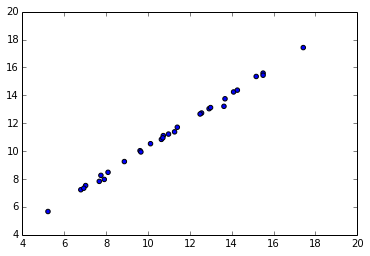
\includegraphics[max size={\textwidth}{\textheight}]{csv-parsing-plotting_files/csv-parsing-plotting_41_1.png}
    \par
    \end{center}
    
            \end{InvisibleVerbatim}
            
        
    


    % Make sure that atleast 4 lines are below the HR
    \needspace{4\baselineskip}

    
        \vspace{6pt}
        \makebox[0.1\linewidth]{\smaller\hfill\tt\color{nbframe-in-prompt}In\hspace{4pt}{[}42{]}:\hspace{4pt}}\\*
        \vspace{-2.65\baselineskip}
        \begin{ColorVerbatim}
            \vspace{-0.7\baselineskip}
            \begin{Verbatim}[commandchars=\\\{\}]
\PY{n}{plot}\PY{p}{(}\PY{n}{weight}\PY{p}{,} \PY{n}{vol}\PY{p}{)}
\end{Verbatim}

            
                \vspace{-0.2\baselineskip}
            
        \end{ColorVerbatim}
    

    

        % If the first block is an image, minipage the image.  Else
        % request a certain amount of space for the input text.
        \needspace{4\baselineskip}
        
        

            % Add document contents.
            
                \makebox[0.1\linewidth]{\smaller\hfill\tt\color{nbframe-out-prompt}Out\hspace{4pt}{[}42{]}:\hspace{4pt}}\\*
                \vspace{-2.55\baselineskip}\begin{InvisibleVerbatim}
                \vspace{-0.5\baselineskip}
\begin{alltt}[<matplotlib.lines.Line2D at 0x44a5710>]\end{alltt}

            \end{InvisibleVerbatim}
            
                \begin{InvisibleVerbatim}
                \vspace{-0.5\baselineskip}
    \begin{center}
    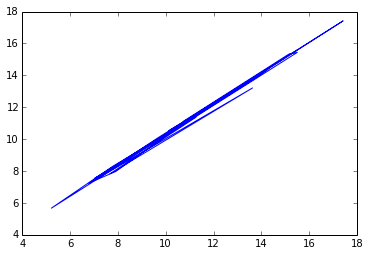
\includegraphics[max size={\textwidth}{\textheight}]{csv-parsing-plotting_files/csv-parsing-plotting_42_1.png}
    \par
    \end{center}
    
            \end{InvisibleVerbatim}
            
        
    
\subsubsection{\href{https://docs.google.com/document/d/1ANWBTbUPTIh\_tL5QjEm4udTCBL0COGJNRzAp5StX5wg/edit?usp=sharing}{Lab
3, Exercise 3}: making your first plot}\subsection{Other types of plots}

\subsubsection{Bar plots}

\begin{itemize}
\item
  http://stackoverflow.com/questions/11617719/how-to-plot-a-very-simple-bar-chart-python-matplotlib-using-input-txt-file
\item
  http://scienceoss.com/bar-plot-with-custom-axis-labels/
\end{itemize}\subsection{Drawing conclusions}

\begin{enumerate}[1.]
\item
  Adding labels
\item
  Writing a sentence summary
\end{enumerate}\subsubsection{Adding labels}

Pretty self-explanatory with the sample code. The things you keep are
the \texttt{plt.figure()} and \texttt{.add\_subplot(111)}. The
\texttt{111} just means that you are adding a subplot to fill the entire
space of the plot window.

    % Make sure that atleast 4 lines are below the HR
    \needspace{4\baselineskip}

    
        \vspace{6pt}
        \makebox[0.1\linewidth]{\smaller\hfill\tt\color{nbframe-in-prompt}In\hspace{4pt}{[}44{]}:\hspace{4pt}}\\*
        \vspace{-2.65\baselineskip}
        \begin{ColorVerbatim}
            \vspace{-0.7\baselineskip}
            \begin{Verbatim}[commandchars=\\\{\}]
\PY{n}{fig} \PY{o}{=} \PY{n}{plt}\PY{o}{.}\PY{n}{figure}\PY{p}{(}\PY{p}{)}
\PY{n}{ax} \PY{o}{=} \PY{n}{fig}\PY{o}{.}\PY{n}{add\PYZus{}subplot}\PY{p}{(}\PY{l+m+mi}{111}\PY{p}{)}
\PY{n}{ax}\PY{o}{.}\PY{n}{set\PYZus{}title}\PY{p}{(}\PY{l+s}{\PYZsq{}}\PY{l+s}{Oyster weight and volume}\PY{l+s}{\PYZsq{}}\PY{p}{)}
\PY{n}{ax}\PY{o}{.}\PY{n}{set\PYZus{}xlabel}\PY{p}{(}\PY{l+s}{\PYZsq{}}\PY{l+s}{Oyster weight (g)}\PY{l+s}{\PYZsq{}}\PY{p}{)}
\PY{n}{ax}\PY{o}{.}\PY{n}{set\PYZus{}ylabel}\PY{p}{(}\PY{l+s}{\PYZsq{}}\PY{l+s}{Oyster volume (cc)}\PY{l+s}{\PYZsq{}}\PY{p}{)}
\PY{n}{ax}\PY{o}{.}\PY{n}{scatter}\PY{p}{(}\PY{n}{weight}\PY{p}{,} \PY{n}{vol}\PY{p}{)}
\PY{c}{\PYZsh{} this saves the figure in a file}
\PY{n}{fig}\PY{o}{.}\PY{n}{savefig}\PY{p}{(}\PY{l+s}{\PYZdq{}}\PY{l+s}{oyster\PYZus{}with\PYZus{}titles.png}\PY{l+s}{\PYZdq{}}\PY{p}{)}
\end{Verbatim}

            
                \vspace{-0.2\baselineskip}
            
        \end{ColorVerbatim}
    

    

        % If the first block is an image, minipage the image.  Else
        % request a certain amount of space for the input text.
        \needspace{4\baselineskip}
        
        

            % Add document contents.
            
                \makebox[0.1\linewidth]{\smaller\hfill\tt\color{nbframe-out-prompt}Out\hspace{4pt}{[}44{]}:\hspace{4pt}}\\*
                \vspace{-2.55\baselineskip}\begin{InvisibleVerbatim}
                \vspace{-0.5\baselineskip}
\begin{alltt}<matplotlib.collections.PathCollection at 0x44db390>\end{alltt}

            \end{InvisibleVerbatim}
            
                \begin{InvisibleVerbatim}
                \vspace{-0.5\baselineskip}
    \begin{center}
    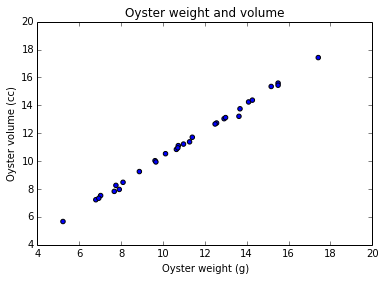
\includegraphics[max size={\textwidth}{\textheight}]{csv-parsing-plotting_files/csv-parsing-plotting_47_1.png}
    \par
    \end{center}
    
            \end{InvisibleVerbatim}
            
        
    
There is a clear relationship between the weight and volumes of oysters
- the bigger the oyster, the heavier it is.
        

        \renewcommand{\indexname}{Index}
        \printindex

    % End of document
    \end{document}


